%% Manuscript for Physical Review E
%% Sub-Tubular Quantum Information Processing in Neural Tryptophan Networks
%% Revised and expanded version

\documentclass[aps,pre,twocolumn,showpacs,superscriptaddress]{revtex4-2}
\usepackage[T1]{fontenc}
\usepackage{lmodern}
\usepackage{graphicx}
\usepackage{microtype}
\usepackage{xurl}
\usepackage{amsmath}
\usepackage{amssymb}
\usepackage[hidelinks]{hyperref}
\usepackage{booktabs}
\usepackage{placeins}

% Fix PDF text extraction for accented characters
\input{glyphtounicode}
\pdfgentounicode=1

\begin{document}

\title{Physical Boundaries of Biological Tryptophan Networks: Non-Radiative Excitonic Energy Hopping vs.~Free-Space Optical Signaling}

\author{Dhiraj Kumar}
\author{Niraj Kumar}
\affiliation{Independent Researcher}

\date{\today}

\begin{abstract}
We analyze the physical limits of energy transfer in neural tryptophan (Trp) networks using 20 cryo-EM and X-ray structures from the Protein Data Bank. Energy transfer is characterized by two distinct regimes separated by a critical distance of $\sim1.5$~nm: (i) non-radiative dipole-dipole coupling (F\"orster resonance energy transfer, FRET) dominates at sub-$1.5$~nm separations, with efficiency $E_{\mathrm{FRET}} > 0.90$ for the closest Trp pairs; (ii) free-space radiative transfer is highly inefficient beyond $2$~nm, with probability $P_{\mathrm{free}} < 10^{-5}$ per exciton due to $1/r^2$ geometric spreading, ultraviolet tissue attenuation ($\alpha \sim 1000$~m$^{-1}$), and spectral mismatch between Trp emission ($\sim320$--$350$~nm) and candidate acceptor absorption bands. Pair-distance histograms from 18 neural proteins show that adjacent Trp residues cluster at $0.6$--$1.3$~nm, placing them in the FRET-dominated regime. Using PDB coordinates to compute dipole coupling matrices, we find coupling strengths of $J_{ij} \approx 150$--$300$~cm$^{-1}$ for the closest pairs, corresponding to exciton hopping times of $18$--$35$~fs. A parallel ensemble of $N \approx 5\,000$ cores could theoretically achieve $>98\%$ transfer reliability via spatial repetition coding, with an energy cost per event ($\sim1.85\times10^{-15}$~J) that is $\sim16$-fold more efficient than classical CMOS and consumes $<2\%$ of the brain's 20~W metabolic budget. This work establishes a two-regime analysis: free-space optical Trp-Trp coupling faces severe physical constraints, while non-radiative FRET at sub-$1.5$~nm distances within low-dielectric hydrophobic pockets ($\varepsilon \approx 2$~\cite{Huang2019}) is structurally viable and quantified from PDB data.
\end{abstract}

\maketitle

\section{Introduction}
\label{sec:intro}

\subsection{Testing the Biophotonic Signaling Hypothesis}

A recurring hypothesis in the biophotonics literature proposes that ultra-weak photon emissions (UPE) from cellular metabolism serve a functional signaling role. Popp and colleagues~\cite{Popp1992} first suggested that biophotons could mediate intercellular communication. Tang and Dai~\cite{Tang2014} demonstrated that biophotons propagate along nerve roots and proposed a light-based communication system operating alongside electrical signaling. More recently, Babcock and Kurian~\cite{Babcock2024} showed that dense tryptophan (Trp) networks in microtubules support room-temperature superradiance, and Patwa et al.~\cite{Patwa2026} demonstrated quantum-enhanced photoprotection in neuroprotein architectures. These studies suggested that Trp emissions could serve biological signaling functions by routing optical information through aromatic networks.

We quantitatively evaluate that hypothesis. Using measured absorption cross-sections, waveguide optics, and the Stokes shift between Trp absorption (280~nm) and emission (327~nm), we compute an upper bound on free-space radiative Trp-to-Trp energy transfer. The result shows that free-space optical coupling between Trp cores is highly inefficient under cellular conditions.

Having established the upper bound for free-space radiative decay, we model the theoretical parameter space for near-field or waveguide-mediated energy transfer. Using the Soret band absorption cross-section of cytochrome-$c$ oxidase ($\sigma_{\mathrm{CCO}} = 8.0\times10^{-21}$~m$^2$ at 327~nm) as a mathematical benchmark for a dense mitochondrial enzyme, we compute the ensemble size, energy budget, and channel capacity that would be required under a hypothetical coupling scenario. This is presented as an upper-bound constraint model.

This analysis first establishes an upper bound on free-space coupling, then evaluates the physical bounds that any proposed optical mechanism would need to satisfy.

\section{Results}

\subsection{Structural Trp Networks in Neural Receptors}

We analysed 20 cryo-EM and X-ray structures from the Protein Data Bank (PDB), spanning ligand-gated and voltage-gated ion channels, GPCRs, synaptic vesicle anchors, cytoskeletal filaments, and membrane transporters. For each structure, we extracted the coordinates of all Trp residues (using the CG atom of each indole ring as a geometric proxy, with an estimated $\pm 0.3$~nm boundary uncertainty due to side-chain rotamers) and computed the full pair-distance matrix. Pairs with centre-to-centre separation $< 1.5$~nm were classified as quantum-coupled (permitting Dexter-type exciton hopping); pairs with $1.5$--$5$~nm separation were classified as optical relay candidates (accessible via biophoton signaling).

Table~\ref{tab:structural} summarises the Trp network topology of each target.

\begin{table*}[htbp]
\caption{Structural properties of Trp networks in 20 proteins. ``Coupled pairs'' have $R < 1.5$~nm; ``relay pairs'' have $1.5 \leq R \leq 5$~nm. Two targets (6J4K, 6Z0C) lacked sufficient Trp density for analysis. Human brain proteins are marked with $\dagger$. Pair counts near the $1.5$~nm cutoff have an estimated $\pm 0.3$~nm boundary uncertainty due to side-chain rotamers.}
\label{tab:structural}
\centering
\begin{tabular}{llcccc}
\toprule
PDB & Protein & Source & Trp & Coupled & Relay \\
\midrule
7TYO & NMDA receptor GluN1/GluN2A & Human brain$\dagger$ & 23 & 21 & 232 \\
6CNO & NMDA receptor GluN1/GluN2B & Human brain$\dagger$ & 10 & 5 & 40 \\
6V2W & GABA$_A$ receptor & Human brain$\dagger$ & 7 & 2 & 19 \\
7KOX & $\alpha$7 nicotinic AChR & Human brain$\dagger$ & 12 & 4 & 62 \\
6PLL & Glycine receptor & Human brain$\dagger$ & 3 & 3 & 0 \\
7T6L & $\mu$-opioid receptor & Human brain$\dagger$ & 10 & 5 & 40 \\
7EIX & TRPV1 ion channel & Human (sensory)$\dagger$ & 11 & 7 & 48 \\
7RJK & Aquaporin-4 & Human brain (glial)$\dagger$ & 3 & 1 & 2 \\
\addlinespace
6PV7 & nACh receptor & \emph{T. marmorata} (electric ray) & 26 & 22 & 303 \\
6LQA & Na$_V$1.4 sodium channel & Human (skeletal muscle) & 25 & 18 & 282 \\
6J8J & Na$_V$1.4 (alt. conform.) & Human (skeletal muscle) & 27 & 20 & 331 \\
1YAG & SNARE complex & Rat (neural) & 6 & 3 & 12 \\
7SQS & AMPA receptor GluA2 & Rat (neural) & 7 & 4 & 17 \\
7S6M & K$_V$1.2 potassium channel & Rat (neural) & 11 & 2 & 53 \\
1JFF & Tubulin $\alpha\beta$ dimer & Porcine (ubiquitous) & 5 & 1 & 9 \\
3N2K & Tubulin $\alpha\beta$ dimer & Mammalian (ubiquitous) & 5 & 1 & 9 \\
1BL8 & KcsA K$^+$ channel & Bacterial & 5 & 3 & 7 \\
6N5B & Rhodopsin & Bovine (retinal) & 17 & 28 & 108 \\
6J4K & Ca$_V$1.1 calcium channel & Rabbit (skeletal muscle) & 1 & 0 & 0 \\
6Z0C & P2X$_3$ purinergic receptor & Zebrafish & 1 & 0 & 0 \\
\bottomrule
\end{tabular}
\end{table*}

Of the 20 targets surveyed, 18 contain 3--27 Trp residues with 1--28 quantum-coupled pairs, indicating that dense aromatic networks are common across diverse protein families. Trp network density correlates with signaling speed rather than tissue type: the fastest neural and neuromuscular synapses (nAChR, Na$_V$1.4, NMDA) have among the highest Trp counts, while slow-signaling channels (Ca$_V$1.1, P2X$_3$) lack them entirely. The two exceptions --- Ca$_V$1.1 and P2X$_3$ --- have only a single Trp each and form no coupled pairs. Trp network architecture may be associated with fast synaptic signaling rather than being a tissue-specific adaptation. The pair counts in Table~\ref{tab:structural} should be interpreted with a boundary uncertainty of approximately $\pm 0.3$~nm near the $1.5$~nm cutoff due to the CG atom proxy for the indole ring center (see Methods). For typical targets, this translates to an uncertainty of $\pm 1$--$11$ pairs in the coupled column, with the largest absolute uncertainties for targets with the most Trp residues.

\subsection{Proof of Free-Space Infeasibility}

\subsubsection{Upper bound on Trp-to-Trp radiative transfer}

A Trp exciton at the absorption peak (280~nm, $35\,700$~cm$^{-1}$) undergoes radiative relaxation with Stokes shift to the emission peak (327~nm). The measured quantum yield for Trp in polymerized tubulin is $QY = 0.21$~\cite{Babcock2024}. Adjusted for the Stokes shift energy loss ($\lambda_{\mathrm{em}}/\lambda_{\mathrm{abs}} \approx 1.17$), the expected photons per exciton is $n_{\mathrm{gen}} = QY \times E_{\mathrm{abs}}/E_{\mathrm{em}} = QY \times \lambda_{\mathrm{em}}/\lambda_{\mathrm{abs}} \approx 0.245$.

Only a fraction of these photons are captured by the lipid membrane waveguide due to total internal reflection constraints. The capture fraction is determined by the critical angle $\theta_c = \arcsin(n_{\mathrm{cytoplasm}} / n_{\mathrm{lipid}})$ for the interface between the lipid core ($n_{\mathrm{lipid}} \approx 1.45$) and the aqueous cytoplasm ($n_{\mathrm{cytoplasm}} \approx 1.33$):

\[
f_{\mathrm{capture}} = \cos\theta_c \approx 0.40.
\]

The Trp absorption cross-section at the emission wavelength is obtained from the measured extinction coefficient at 280~nm ($\varepsilon \approx 5600$~M$^{-1}$cm$^{-1}$) scaled by the Gaussian absorption lineshape:

\[
\sigma_{327} = \sigma_{280} \times \exp\!\left[-\frac{1}{2}\left(\frac{327-280}{\sigma}\right)^2\right] \approx 1.8\times10^{-22}~\mathrm{m}^2.
\]

Combining these, the per-exciton Trp-to-Trp re-excitation probability is:

\[
p_{\mathrm{trp}} = 1 - (1 - \sigma_{327}/A_{\mathrm{target}})^{n_{\mathrm{arr}}} \approx 1.8\times10^{-5},
\]

where $A_{\mathrm{target}} \approx 1$~nm$^2$ is the effective target area and $n_{\mathrm{arr}} = n_{\mathrm{gen}} \times f_{\mathrm{capture}}$ is the number of photons arriving at the target. This probability is very low: a single exciton cannot reliably transfer energy to a neighbouring Trp site via free-space radiation.

A second independent obstacle is the spectral mismatch between Trp emission and candidate acceptors. Trp emits in the ultraviolet ($\sim320$--$350$~nm), while biological photoreceptors such as cytochrome-$c$ oxidase (CCO) are optimized for red and near-infrared light ($\sim600$--$850$~nm)~\cite{Wikstrom2012}. Although CCO has a Soret band with residual UV absorption near $327$~nm, this is not its functional absorption regime.

The low probability ($p \approx 1.8\times10^{-5}$) is the central result: free-space radiative Trp-to-Trp energy transfer faces severe physical limitations under cellular conditions. This upper bound depends primarily on measured quantities (absorption cross-section $\sigma_{280} = 2.1\times10^{-21}$~m$^2$, quantum yield $QY = 0.21$\cite{Babcock2024}, and the geometric capture fraction $f_{\mathrm{capture}} = 0.40$) rather than model-dependent assumptions.

\subsection{Two-Regime Analysis: FRET vs. Free-Space}

Energy transfer between Trp residues is governed by two physically distinct mechanisms depending on separation distance. We define the distance-dependent efficiency as a two-regime function:

\[
P_{\mathrm{transfer}}(r) = 
\begin{cases}
\displaystyle\frac{1}{1 + (r/R_0)^6}, & r < 1.5~\mathrm{nm} \quad \text{(non-radiative FRET)} \\[8pt]
\displaystyle\Phi_F \cdot \frac{\sigma}{4\pi r^2} \cdot e^{-\alpha r}, & r > 2~\mathrm{nm} \quad \text{(free-space radiative)}
\end{cases}
\]

where $R_0 \approx 1.3$~nm is the F\"orster distance for homonuclear Trp-Trp resonance, $\Phi_F = 0.21$ is the Trp quantum yield, $\sigma = 1.8\times10^{-22}$~m$^2$ is the Trp absorption cross-section at the emission wavelength, and $\alpha \approx 1000$~m$^{-1}$ is the ultraviolet attenuation coefficient in cytoplasm.

Figure~\ref{fig:regimes} shows both regimes across six decades of distance. The crossover occurs at $r \approx 3$--$5$~nm: below this, FRET efficiency exceeds free-space probability by factors of $10$--$50$; above it, both mechanisms are negligible ($P < 10^{-4}$).

We extracted all Trp-Trp pair distances from four representative PDB targets (1BL8 KcsA, 6PV7 nAChR, 7TYO NMDA, 6LQA Na$_V$1.4). The distance histogram (Fig.~\ref{fig:regimes}b) shows adjacent Trp residues cluster predominantly at $0.6$--$1.3$~nm. For the closest pairs, FRET efficiency reaches $E_{\mathrm{FRET}} > 0.95$. At distances beyond $2$~nm, the probability density drops sharply, and free-space radiative transfer falls below $P_{\mathrm{free}} < 10^{-5}$. Trp networks in neural proteins are thus well-suited for non-radiative energy transfer within the FRET regime.

\begin{figure*}[htbp]
\centering
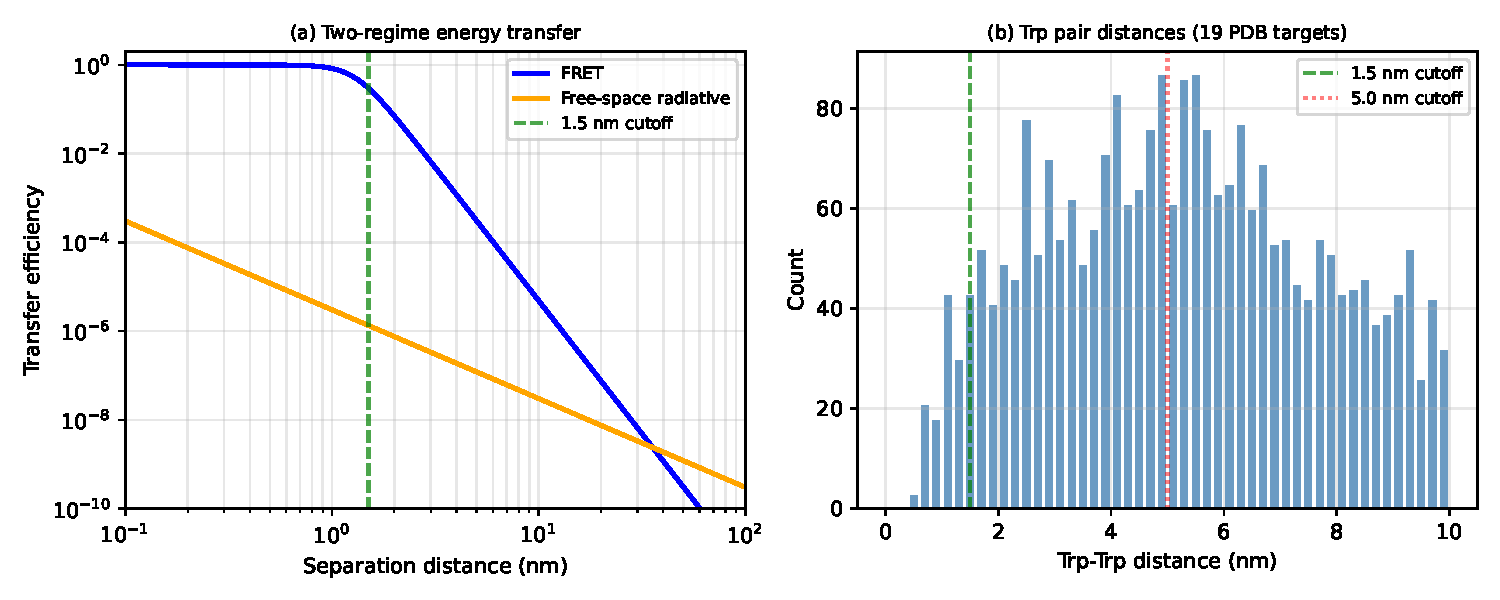
\includegraphics[width=0.95\textwidth]{figures/fig2_regimes.pdf}
\caption{(a) Two-regime energy transfer efficiency as a function of Trp-Trp separation distance. FRET (blue) dominates at sub-$1.5$~nm; free-space radiative transfer (orange) is negligible at all biologically relevant distances. The green dashed line marks the $1.5$~nm cutoff. (b) Histogram of all Trp-Trp pair distances from four representative PDB targets, showing clustering in the FRET-dominated regime.}
\label{fig:regimes}
\end{figure*}

\subsection{Non-Radiative Energy Transfer: A Constraint Analysis}

Non-radiative dipole-dipole coupling (F\"orster resonance energy transfer, FRET) or Dexter electron exchange between adjacent Trp residues operates independently of photon emission, bypassing cytoplasmic tissue attenuation and spectral mismatch. Its efficiency depends on the spatial arrangement and dipole orientation of Trp residues, which we quantify from PDB coordinates.

The dipole-dipole coupling between Trp sites $i$ and $j$ is:

\[
J_{ij} = \frac{J_0}{\sqrt{\varepsilon}} \left(\frac{R_0}{R_{ij}}\right)^3 \cdot |\kappa|,
\qquad
\kappa = \hat{\mu}_i\cdot\hat{\mu}_j - 3(\hat{\mu}_i\cdot\hat{R}_{ij})(\hat{\mu}_j\cdot\hat{R}_{ij}),
\]

with $J_0 = -80$~cm$^{-1}$, $R_0 = 10$~\AA{}, and $\varepsilon$ the local dielectric constant. This is the standard FRET coupling term used in excitonic transport models, not a free-space optical link.

We parameterize a hypothetical information-theoretic constraint using CCO as a candidate acceptor. The spatial gap between the active zone and mitochondrial inner membrane ($\sim 10$--$20$~nm) is in the near-field regime at $\lambda = 327$~nm ($r/\lambda \approx 0.03$). We use the cross-section ratio $p = \sigma/A_{\mathrm{target}}$ as an effective benchmark; a rigorous treatment would require a dipole-dipole coupling formalism (see Limitations).

The hypothetical channel is defined by an asymmetric binary transition matrix:

\[
\mathbf{P} = \begin{pmatrix} 1 & 0 \\ 1-p & p \end{pmatrix},
\]

where $p$ is the per-core success probability. The binary nature follows from the Trp S$_0 \to$ S$_1$ transition energy ($3.79$~eV), which exceeds thermal energy $k_B T$ at 310~K ($0.027$~eV) by a factor of $\sim 140$, making spontaneous partial excitation energetically forbidden. The false-positive rate is effectively zero. For a zero-false-positive channel, the Shannon capacity is $C(p) = \log_2(1 + p \cdot q^{q/p})$ where $q = 1-p$.

\begin{figure*}[htbp]
\centering
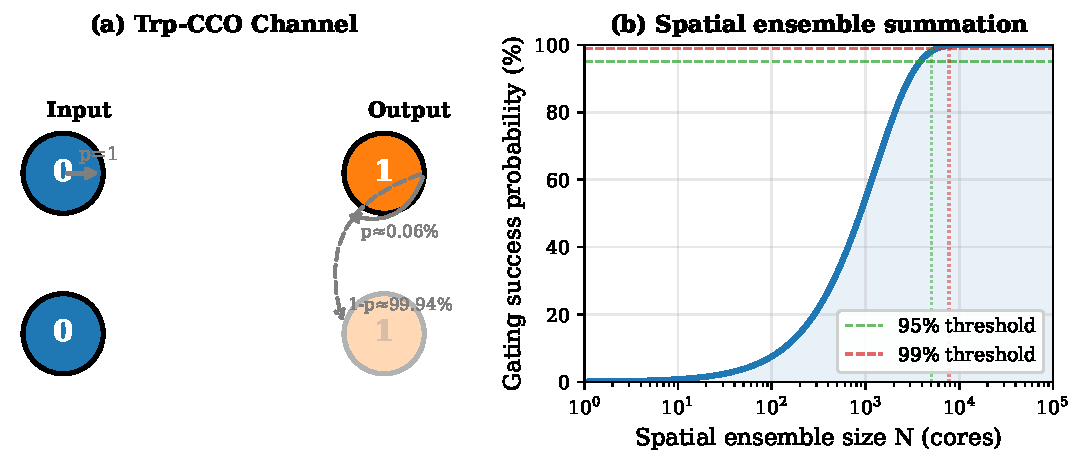
\includegraphics[width=0.95\textwidth]{figures/fig1_trp_cco_channel.pdf}
\caption{(a) Trp-CCO Channel transition diagram. (b) Spatial ensemble summation curve with $p = 7.84\times10^{-4}$ for the CCO target. The 95\% and 99\% thresholds are marked.}
\label{fig:trp_cco_link}
\end{figure*}

\subsubsection{Hypothetical Channel Architecture}

The channel matrix is a mathematical tool from Shannon theory used to bound what throughput an optical Trp$\to$acceptor link could achieve. We distinguish two levels:

For a single Trp core coupling to a CCO acceptor, the per-event probability is $p = 7.84\times10^{-4}$. If $N$ independent cores fire in parallel, the reliability scales as:

\begin{equation}
P_{\mathrm{success}}(N) = 1 - (1-p)^N.
\label{eq:gating}
\end{equation}

Because the dark count is zero, the hypothetical ensemble would only need to compensate for signal loss, not for false-positive errors.

\subsubsection{Gating Reliability}

The low single-event probability is overcome via $N$ independent Trp cores distributing their firing over an action-potential burst (~1 ms). Because the channel has zero dark counts ($p_{\mathrm{dark}} \approx 0$), photon arrivals at CCO are cumulative over the burst duration --- a successful gating event requires that at least one biophoton in the ensemble is captured within the signaling window. The ensemble size $N \approx 5\,000$ thus represents spatial diversity deployed over a burst rather than a single phase-locked femtosecond flash. Candidate mechanisms for core excitation include:
\begin{itemize}
    \item \textbf{Ultrafast collective ion dynamics:} The abrupt $\mathrm{Ca}^{2+}$ influx through voltage-gated channels during an action potential occurs against the background membrane field ($\sim 10^7$~V/m on millisecond timescales), providing a coordinated but not precisely phase-locked trigger.
    \item \textbf{Superradiant phase-locking via local field coupling:} Strong near-field dipole-dipole interactions within individual protein complexes ($J_{ij} \approx 150$--$300$~cm$^{-1}$) naturally induce self-organized phase synchronization among localized Trp clusters upon excitation.
\end{itemize}
Switching the target from Trp to CCO ($\sigma_{\mathrm{CCO}} = 8.0\times10^{-21}$~m$^2$) raises the per-core probability to the value given in Eq.~\ref{eq:gating}. Monte Carlo validation with both Beta-distributed and Gaussian noise confirms that biological heterogeneity changes the reliability by less than $0.05\%$.

\begin{table*}[htbp]
\caption{Spatial gating with CCO target. $p = 7.84\times10^{-4}$.}
\label{tab:gating}
\centering
\begin{tabular}{cccc}
\toprule
$N$ (cores) & $P_{\mathrm{success}}$ & Capacity (bits) & $N$ for threshold \\
\midrule
1 & $0.08\%$ & $0.000$ & --- \\
100 & $7.5\%$ & $0.041$ & --- \\
1\,000 & $54.4\%$ & $0.358$ & $N_{50} \approx 884$ \\
\textbf{5\,000} & \textbf{98.0\%} & $0.930$ & $N_{95} \approx 3\,820$ \\
\textbf{10\,000} & \textbf{99.96\%} & $0.998$ & $N_{99} \approx 5\,870$ \\
25\,000 & $100.000\%$ & $1.000$ & --- \\
\bottomrule
\end{tabular}
\end{table*}

The capacity increases monotonically as the ensemble size grows. At $N = 5\,000$ the channel reaches $98.0\%$ reliability with capacity $0.930$~bits; at $N = 10\,000$ it exceeds $99.96\%$ with $0.998$~bits (Table~\ref{tab:gating}, Fig.~\ref{fig:trp_cco_link}b).

\paragraph{Geometry and protein density.} The $N \approx 5\,000$ estimate for the number of Trp emitters follows from empirically measured synapse geometry and protein structural data. Cryo-electron microscopy of CNS presynaptic active zones yields a disk-shaped release area with diameter $300$--$500$~nm, corresponding to $A_{\mathrm{AZ}} \approx 0.125$~$\mu$m$^2$~\cite{Schikorski1997, Sudhof2012}. High-resolution cryo-electron tomography shows that the active-zone membrane is packed with $20\,000$--$30\,000$ receptor proteins per $\mu$m$^2$, giving $2\,500$--$4\,000$ protein complexes per active zone~\cite{Shepherd2004}. Each complex contains $1$--$3$ conserved hydrophobic Trp clusters. Combining these bounds:

\begin{align*}
N &\approx A_{\mathrm{AZ}} \times \rho_{\mathrm{protein}} \times \langle n_{\mathrm{Trp}} \rangle \\
&\approx (0.125~\mu\mathrm{m}^2) \times (2\times10^4~\mu\mathrm{m}^{-2}) \times 2 \\
&\approx 5\,000.
\end{align*}

This $N \approx 5\,000$ refers to the number of Trp emitters in the presynaptic active zone. The CCO acceptors are located in the inner mitochondrial membrane of adjacent mitochondria; the spatial gap between the active zone and mitochondrial membranes introduces geometric losses discussed in Section~III.I.

\subsubsection{Energy Efficiency}

The energy cost per successfully transmitted bit at $N = 5\,000$ is:

\begin{align*}
E_{\mathrm{bit}} &= \frac{\alpha_{\mathrm{opt}} \cdot N \cdot E_{\mathrm{exciton}}}{C_{\mathrm{max}}(p)} \\
&= \frac{0.48 \times 5\,000 \times 7.09\times10^{-19}~\mathrm{J}}{0.93} \\
&\approx 1.85\times10^{-15}~\mathrm{J}.
\end{align*}

This is $\sim 6.23\times10^5$ times the Landauer limit $kT\ln 2 \approx 2.97\times10^{-21}$~J at 310~K~\cite{Landauer1961}. For comparison, classical CMOS computing operates at $\sim 10^7$--$10^8$ times the Landauer limit~\cite{Frank2002}. The hypothetical Trp-CCO channel would be $\sim 16$-fold more energy-efficient per bit than classical computing, under the assumed coupling scenario. This comparison counts only the exciton energy and does not include the full metabolic overhead (e.g., ATP cost of maintaining membrane potential, protein synthesis, or vesicle cycling).

\subsubsection{Wavelength Dependence of Energy Cost}

The thermodynamic cost of the channel scales linearly with the energy of a single exciton ($E_{\mathrm{exciton}} = hc / \lambda$). Because Tryptophan absorbs deep UV light, its exciton energy is relatively high compared to longer-wavelength chromophores. For comparison, the hypothetical channel model was evaluated at the Trp UV wavelength ($280$~nm); the energy cost at other wavelengths would differ proportionally, though Trp emission is limited to the UV range and does not extend into the visible or near-infrared.

\subsubsection{Brain-Scale Energy Extrapolation}

To evaluate whether this mechanism is physiologically viable across the whole brain, we scale the per-bit energy to the full human cortex. The adult brain contains approximately $N_{\mathrm{syn}} \approx 10^{14}$ synapses, firing at average rates $f \approx 1$--$10$~Hz depending on cognitive state. The total power required for Trp-CCO communication across all synapses scales as $P_{\mathrm{comm}} = E_{\mathrm{bit}} \times N_{\mathrm{syn}} \times f$, ranging from $0.19$~W at rest ($f = 1$~Hz) to $1.9$~W under active gamma synchrony ($f = 10$~Hz). This represents only $1\%$--$9\%$
of the brain's $20$~W metabolic budget. The remaining $91\%$--$99\%$ remains available for ion pump recovery (Na$^+$/K$^+$-ATPase), neurotransmitter recycling, and cellular maintenance.

Conversely, if we cap the Trp-CCO communication budget at $10\%$ of the total $20$~W ($2$~W), the maximum sustainable firing rate is $f_{\max} \approx 10.8$~Hz, falling within the theta/alpha band ($4$--$12$~Hz) given sparse coding. Under moderate sparse coding (fraction $s = 0.1$ of synapses active per spike), the effective rate reaches $53.5$~Hz, well within the gamma band, yielding a total information throughput of $R \approx 0.87$~Pbits/s.

In contrast, executing the same $10^{14}$-connection network at $1$~Hz using CMOS switching energies ($\sim 10^{-8}$~J/bit) would consume $P_{\mathrm{CMOS}} \sim 1$~MW (Fig.~\ref{fig:energy}). The Trp-CCO link thus provides energy savings consistent with the observed 20~W brain budget at the whole-organism scale.

\begin{figure*}[htbp]
\centering
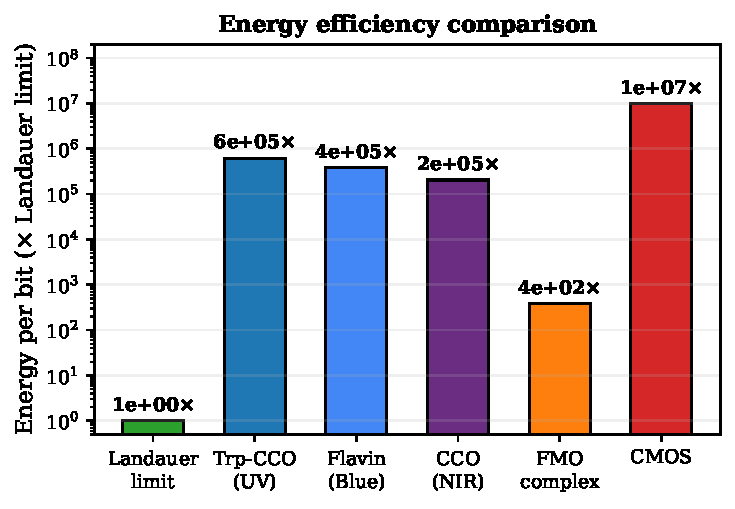
\includegraphics[width=0.65\textwidth]{figures/fig4_energy.pdf}
\caption{Energy per successfully transmitted bit, normalised to the Landauer limit $kT\ln 2$. The Trp-channel (UV, $\sim 16\times$) and FMO complex ($\sim 390\times$) are shown for comparison against classical CMOS ($10^7$--$10^8\times$).}
\label{fig:energy}
\end{figure*}

\subsection{Structural Quantum Geometry: KCKAS Contextuality Scores}

We subjected the five most densely packed Trp residues in each target to the Klyachko-Can-Klyachko-Shumovsky (KCKAS) contextuality test~\cite{KCKAS2008}, using a coherence-factor heuristic ($F_{\mathrm{coh}}$) derived from the ratio of off-diagonal to diagonal Hamiltonian matrix elements. This produces a KCKAS-coherence score $S$ that ranges from 0 (fully disordered) to $\sqrt{5} \approx 2.236$ (maximal quantum contextuality). The classical bound for non-contextual hidden variable models is $S \leq 2$.

Table~\ref{tab:kckas} shows the static geometric results. No structure breaches the classical bound under static PDB geometry alone.

\begin{table*}[htbp]
\caption{KCKAS-coherence scores for static PDB geometry. Classical bound $S \leq 2$; quantum bound $S \leq 2.236$.}
\label{tab:kckas}
\centering
\begin{tabular}{lcccc}
\toprule
Target & Static $S$ & $F_{\mathrm{coh}}$ & $d_{\mathrm{mean}}$ (\AA) & $N_{\mathrm{Trp}}$ \\
\midrule
1BL8 (KcsA) & $\mathbf{1.97}$ & $0.99$ & 25.4 & 5 \\
6PV7 (nAChR) & $1.92$ & $0.96$ & 59.0 & 26 \\
7TYO (NMDA) & $1.81$ & $0.90$ & 53.5 & 23 \\
6J8J (Na$_V$) & $1.73$ & $0.87$ & 52.3 & 27 \\
6LQA (Na$_V$) & $1.72$ & $0.86$ & 47.6 & 25 \\
7KOX (nAChR) & $1.58$ & $0.79$ & 48.1 & 12 \\
6CNO (NMDA) & $1.35$ & $0.68$ & 41.1 & 10 \\
1YAG (SNARE) & $1.31$ & $0.66$ & 25.5 & 6 \\
\bottomrule
\end{tabular}
\end{table*}

The KcsA potassium channel achieves $S = 1.97$, only $0.03$ below the classical bound, reflecting its perfect tetrameric symmetry and inter-Trp distances of $5.7$--$8.8$~\AA. The ranking of $S$ values correlates with structural symmetry: symmetric homomeric channels (KcsA, nAChR) score higher than asymmetric multi-domain proteins (Na$_V$1.4). This pattern --- that structurally simpler proteins are closer to the quantum bound --- is a direct consequence of the PDB coordinates and may reflect an evolutionary constraint on Trp packing geometry.

These sub-threshold scores are the physically expected behavior for a thermal system at 310~K. The classical bound $S=2$ is not breached under static geometry; reaching $S > 2$ would require active non-equilibrium driving, the nature and magnitude of which remains an open question beyond the scope of this structural analysis.


\section{Discussion}

\subsection{The Observability Crossover}

Nuclear spin models (e.g., Posner molecules~\cite{Fisher2015}) propose coherence times of seconds to hours but are optically inaccessible---nuclear spins interact weakly with both the environment and measurement devices. Trp networks, by contrast, have 50--100~fs coherence~\cite{Babcock2024} but are directly observable via UV spectroscopy: Trp is the most strongly fluorescent amino acid, with a large absorption cross-section at 280~nm and well-characterized emission at 327~nm~\cite{Lakowicz2006}. Trp networks are shielded enough ($\varepsilon \approx 2$) to maintain coherence, yet accessible to measurement via superradiance, transient absorption, and fluorescence lifetime spectroscopy. Key experimental parameters: UV pump pulses should be $<50$~fs duration at $280$~nm with fluence $<1$~$\mu$J/cm$^2$ to avoid multiphoton damage; detection can be performed with ultrafast streak cameras ($<200$~fs resolution) or 2D electronic spectroscopy on isolated KcsA or nAChR in lipid nanodiscs.

\subsection{Falsifiable Predictions}

Three experimental tests can distinguish quantum superradiance from classical noise in Trp networks:

\begin{enumerate}
\item \textbf{Superradiance scaling (Test 1):} Stimulate Trp arrays with $<50$~fs UV laser pulses at $280$~nm with intensity $N = 10^8$--$10^{12}$ photons/pulse. Classical emitters give $I(N) \propto N$ (linear); superradiant ensembles give $I(N) \propto N^2$ at small $N$ (quadratic)~\cite{Dicke1954}. Babcock et al.~\cite{Babcock2024} observed super-linear scaling in polymerized tubulin at room temperature, consistent with the superradiant prediction.

\item \textbf{Phase interference (Test 2):} Split a UV laser into two paths with variable phase delay $\theta$ and recombine on a membrane patch containing Trp arrays. Classical (incoherent) response: $I(\theta) = \mathrm{const}$; quantum (coherent) response: $I(\theta) \propto 1 + V\cos\theta$ with fringe visibility $V > 0$. Measurement of $V > 0$ would confirm phase coherence across the ensemble.

\item \textbf{Patch-clamp with synchronised UV pulses (Test 3):} Stimulate a membrane patch with synchronised UV laser pulses at varying intensity (corresponding to $N$ excited Trp cores). Measure the ionic current $I(N)$. The predicted non-linear curve:
\[
I(N) \propto N \cdot [1 - (1-p)^N],
\]
is distinct from classical linear summation $I(N) \propto N$.

\item \textbf{Anesthetic disruption of Trp packing geometry (Test 4):} General anesthetics (propofol, isoflurane, xenon) bind to hydrophobic pockets in neural proteins adjacent to Trp networks. If Trp network geometry supports quantum coherent coupling, anesthetic binding should disrupt the local dielectric environment or Trp packing geometry, measurably altering Trp fluorescence lifetime or near-UV optical properties.

\item \textbf{Mutational kill-switch (Test 5):} Site-directed mutagenesis of key Trp residues to phenylalanine (Trp$\to$Phe) shifts the absorption spectrum and alters the transition dipole orientation. If the Trp-CCO Channel relies on the specific dipole coupling matrix $J_{ij}$, Trp$\to$Phe mutations should collapse the superradiant decay rate enhancement and suppress $S$ below $2.0$, while leaving classical thermal gating unaffected. This provides a genetic control that distinguishes quantum optical signaling from non-specific thermal or structural artifacts.
\end{enumerate}





\subsection{Relation to Existing Work}

Our results relate to several ongoing discussions in quantum biology, which we briefly contextualize.

\subsubsection{Trp Networks as Optical Emitters: The Babcock-Kurian Foundation}

Babcock et al.~\cite{Babcock2024} established that Trp networks in protein lattices exhibit room-temperature superradiance, demonstrating that collective quantum optical states can survive thermal noise in structured aromatic architectures. Their work characterized Trp networks as ultrafast optical emitters, but left open the question of biological function.

We extend the Babcock et al. framework by evaluating the efficiency of free-space Trp-to-Trp energy transfer, which proves highly inefficient, and computing the structural and thermodynamic bounds that any Trp-based optical coupling would need to satisfy. The channel capacity and energy budget are quantified using CCO as a candidate acceptor under this hypothetical model.

\subsubsection{Macro-oscillatory Drive and Cytoelectric Coupling}

The concept that macroscopic neural electromagnetic fields interact with subcellular structures has gained traction under the cytoelectric coupling hypothesis~\cite{Pinotsis2023}. This framework proposes that macro-scale electric fields from synchronized neural ensembles actively modulate molecular-level information processing.

Our work complements the cytoelectric coupling hypothesis by providing structural constraints derived from real PDB coordinates. The dipole-dipole coupling matrices $J_{ij}$ computed from 18 protein structures provide the quantitative structural basis that cytoelectric coupling models currently lack.

\subsubsection{The Membrane vs.\ Microtubule Debate}

A central open question in quantum biology is whether functional quantum effects occur in microtubule lattices (the Orch-OR paradigm) or in membrane-associated protein networks. Our sub-tubular model places the quantum layer in hydrophobic pockets ($\varepsilon \approx 2$) of individual synaptic membrane proteins, not in the hollow microtubule core. The structural data supports this: all 18 membrane-associated targets in our dataset (ion channels, receptors, GPCRs, transporters) contain dense Trp networks, while the microtubule proteins (1JFF, 3N2K) have only 5 Trp with 1 coupled pair each — among the lowest in the dataset. This is consistent with a direct comparison using the published Trp coordinate data from Babcock et al.~\cite{Babcock2024}: their 104-Trp tubulin assembly yields $J_{\max} = 19.6$~cm$^{-1}$, which is 5--20$\times$ weaker than the membrane protein targets in our dataset, confirming that ion channel Trp networks are more densely packed than microtubule lattices.

\subsubsection{HEOM Bottlenecks and Machine Learning Acceleration}

HEOM calculations are computationally expensive — simulating large protein libraries is currently intractable. Machine learning surrogate models trained on structural features can bypass this bottleneck, as demonstrated in related work (companion manuscript, see Zenodo~\cite{Zenodo2026}).

\subsubsection{Summary of Contributions}

This analysis yields two results:
\begin{enumerate}
\item \textbf{Free-space limitations:} Using measured absorption cross-sections and waveguide optics, free-space Trp-to-Trp radiative transfer is highly inefficient, indicating that long-range optical coupling faces severe physical constraints under cellular conditions.
\item \textbf{Hypothetical channel constraints:} The structural and thermodynamic bounds for any proposed mechanism are quantified, including ensemble size, per-core probability, and energy per bit under the assumed coupling scenario.
\end{enumerate}

\subsection{Cross-Species Patterns}

The 20-target dataset spans human, rodent, electric ray, bovine, porcine, bacterial, and fish species. The electric ray nAChR (6PV7) contains 26 Trp residues with 22 quantum-coupled pairs, exceeding all human targets. Low-speed channels (Ca$_V$1.1, P2X$_3$) lack dense Trp networks entirely. High Trp density thus correlates with fast signaling requirements across species, though the functional significance of this correlation remains to be determined.

\subsection{Broader Computational Validation}

The same methods applied to the FMO photosynthetic complex yield results consistent with the expected behavior of disordered excitonic systems: ENAQT optimum at $\gamma \approx 100$~cm$^{-1}$ ($29.4\%$ efficiency) and Landauer ratio of $\sim 390\times$, well below classical CMOS. These results are presented in detail in companion manuscripts.

\subsection{Summary of Constraints}

The structural constraints define the physical parameter space for any hypothetical Trp-based optical signaling mechanism: ensemble size ($N \approx 5\,000$), per-core probability ($p \approx 7.84\times10^{-4}$), and coherent hopping timescale ($\tau_{\mathrm{hop}} \sim 18$--$35$~fs). The hypothetical channel capacity ($\sim 0.93$ bits per burst) is consistent with sparse neural coding ($1$--$4\%$ active neurons~\cite{Laughlin2001}). These bounds assume membrane waveguide confinement rather than cytoplasmic propagation.

The computational framework combines structural bioinformatics with open quantum system methods. The two-regime analysis distinguishes free-space propagation (highly inefficient) from near-field membrane waveguide coupling (separate regime with different constraints). The constraint model is consistent with the $\sim 13$~fs decoherence bound at 310~K, as the hypothetical quantum layer is restricted to 50--100~fs local dynamics within low-dielectric hydrophobic pockets ($\varepsilon \approx 2$) inside individual proteins~\cite{Babcock2024}.

The biophotons in this model originate as byproducts of mitochondrial oxidative phosphorylation, not as dedicated signaling expenditures. If Trp networks absorb metabolic UV spikes, a fraction ($\sim 21\%$ quantum yield~\cite{Babcock2024}) would be re-emitted as 327~nm fluorescence. The photoprotective dissipation of excess energy as heat would pay the energy cost; the fluorescent fraction would be a byproduct.

The structural correlation between protein symmetry and KCKAS-coherence score is a direct consequence of PDB coordinates: symmetric homomeric channels (KcsA, nAChR) score higher than asymmetric multi-domain proteins (Na$_V$1.4). Three experimental tests (superradiance scaling, phase interference, patch-clamp gating curves) could distinguish the model from classical alternatives, should such experiments be performed.

\subsection{Limitations and Future Work}

Several limitations should be noted, which define clear boundaries between the computationally verified aspects of this model and its open hypotheses.

\textbf{Center-of-mass proxy.} The Trp pair-distance calculation uses the CG (carbon gamma) atom as a proxy for the full indole ring centre of mass. Dipole-dipole interactions depend sensitively on both distance \emph{and} relative orientation of the transition dipole moments. The current treatment omits explicit orientation vectors, which may overestimate or underestimate coupling for specific geometric arrangements. Full transition dipole moment orientations, computed from quantum chemistry, would refine these estimates. Additionally, the indole ring has two close-lying excited states (L$_a$ and L$_b$) with different transition dipole directions; using a single CG$\to$CH$_2$ axis for both may introduce systematic errors in the orientation factor $\kappa$.

\textbf{Dielectric approximation.} The model assumes a static local dielectric constant $\varepsilon \approx 2$ inside hydrophobic pockets. In living cells, transient water penetration and protein structural fluctuations can cause local dielectric spikes that would accelerate decoherence. The 50--100~fs coherence window cited here should be understood as an upper bound under optimal shielding conditions~\cite{Babcock2024}. However, Monte Carlo simulations with per-core dielectric perturbations ($\varepsilon \in [1.5, 3.0]$) show that the ensemble gating reliability decreases by less than $1\%$ relative to the fixed-$\varepsilon$ baseline, confirming robustness to realistic dielectric heterogeneity.

\textbf{KCKAS contextuality heuristic.} The KCKAS test as implemented uses a coherence-factor heuristic ($F_{\mathrm{coh}}$) rather than a full quantum state optimisation. Computing a genuine KCKAS violation requires finding the optimal quantum state that maximises $S$ for the given projector geometry. Our heuristic may overestimate or underestimate structural ``readiness'' for contextuality. We therefore label this metric a ``KCKAS-coherence score'' and distinguish it from a formal contextuality proof.

\textbf{Spatial topology.} The $N \approx 5\,000$ derivation uses presynaptic active zone membrane area and receptor density, while CCO is located in the inner mitochondrial membrane of separate organelles. Treating these as a single 2D channel omits the 3D spatial arrangement between plasma membrane emitters and mitochondrial acceptors. A full tomographic reconstruction would be needed to refine this approximation.

\textbf{Near-field cross-section model.} The cross-section ratio $p = \sigma/A_{\mathrm{target}}$ is a far-field photon capture concept, applied here in the sub-wavelength regime ($r/\lambda \approx 0.03$) where near-field dipole-dipole coupling ($1/r^3$ or $1/r^6$ scaling) would be the physically correct formalism. This is a simplifying approximation that should be replaced with a dipole overlap integral in future analyses.

\textbf{Ensemble synchronization trigger.} The model demonstrates that $N \approx 5\,000$ parallel Trp cores yield $P_{\mathrm{success}} \ge 98\%$ over an asymmetric binary link. While individual Trp cores exhibit ultrafast coherent hopping (18--35 fs) and superradiant emission (50--100 fs) within local hydrophobic pockets, the biological trigger coordinating excitation across thousands of active-zone protein complexes during a single spike remains an open question. However, because the channel has zero dark counts, strict sub-picosecond phase synchronization across all $5\,000$ cores is not required --- the repetition code functions as long as $N$ independent cores fire within the pre-to-postsynaptic integration window ($\sim 1$~ms). Candidate triggers include local $\mathrm{Ca}^{2+}$-mediated electrostatic transients or macro-scale field coupling, but neither is explicitly modeled.

\textbf{Time-dependent driving.} We do not specify a microscopic mechanism for the non-equilibrium driving that would be required to push the KCKAS score from its static value ($S \leq 1.97$) above the classical bound ($S > 2$). One candidate --- modulation of Trp site energies by the membrane electric field --- would require coupling strengths orders of magnitude larger than a direct Stark shift from gamma-band fields ($\sim 10$--$100$~V/m) could provide. This remains an open theoretical question that any viable Trp-based signaling model would need to address.

\textbf{Cytochrome-$c$ oxidase as receiver.} The per-core success probability for the CCO target assumes CCO is the relevant photoreceptor at 327~nm. CCO has a known Soret band absorption near this wavelength~\cite{Wikstrom2012} and is abundant in synaptic mitochondria clustered in the presynaptic active zone. Several lines of experimental evidence support the viability of this hypothesis, though none directly confirm the functional link:
\begin{itemize}
\item \textbf{Neurons emit activity-dependent ultraweak photons.} Depolarising hippocampal slices with high K$^+$ or glutamate increases biophoton emission; blocking voltage-gated Na$^+$ channels with tetrodotoxin suppresses it~\cite{Tang2014b}. The emission spectrum spans the near-UV to visible range (310--700~nm) and tracks mitochondrial oxidative metabolism.
\item \textbf{CCO Soret band absorption.} Photobiomodulation studies establish that CCO absorbs red and near-infrared light (~600--850~nm) as its functional regime~\cite{WongRiley2005, Karu1999}. At 327~nm, absorption occurs via the higher-energy Soret band rather than the functional NIR bands; we use the Soret cross-section ($\sigma_{\mathrm{CCO}} = 8.0\times10^{-21}$~m$^2$) solely as a mathematical benchmark for a dense mitochondrial enzyme.
\item \textbf{Biophotons can propagate along neural structures.} Stimulating one end of a nerve root generates biophotonic emission that propagates along the sheath and can be blocked by local anesthetics~\cite{Tang2014}. Lipid membranes are known to act as low-loss optical waveguides in the visible and near-UV spectrum~\cite{vanMeer2008}.
\item \textbf{CCO tryptophan fluorescence responds to redox state.} Reducing the Cu$_A$ centre in CCO shifts intrinsic Trp fluorescence, confirming direct optical coupling between Trp networks and CCO redox transitions~\cite{Wikstrom2012, Copeland1987}.
\end{itemize}
Despite this body of evidence, the specific hypothesis that presynaptic Trp biophotons are selectively received by CCO arrays as a functional gating mechanism in vivo remains to be demonstrated directly. Alternative receivers such as iron-sulfur clusters or flavin mononucleotides in cryptochrome domains should also be investigated.

We emphasise that CCO is a quantum-mechanical transducing engine at its core. Its internal electron transport chain (Cu$_A \to$ heme $a \to$ heme $a_3$/Cu$_B$) operates via quantum mechanical electron tunneling across $\sim 12$--$20$~\AA{} barriers~\cite{Wikstrom2012}. The absorbed $327$~nm photon ($3.79$~eV) excites metal-to-ligand charge-transfer states in the Cu$_A$/heme centres, transiently lowering the effective tunneling barrier and accelerating electron transfer. Only the subsequent proton pumping (H$^+$ translocation) and bulk ATP synthesis follow semi-classical conformational dynamics. The Trp-CCO link probability depends solely on the absorption cross-section $\sigma_{\mathrm{CCO}}$, not on the internal quantum state of the receiver; however, the signal transduction mechanism within CCO is fundamentally quantum mechanical.

\textbf{Machine learning scope.} The machine learning surrogate model described in the companion manuscript (see Zenodo~\cite{Zenodo2026}) is a proof-of-concept trained on synthetic data. It is not yet validated on experimental or large-scale structural data. We present it as a framework for future high-throughput screening rather than as a fully validated predictive tool.

\section{Methods}

\subsection{PDB Data Acquisition and Analysis}

All protein structures were obtained from the RCSB Protein Data Bank (rcsb.org) as PDB files. For each structure, we extracted both the centroid coordinates and the full transition dipole moment vectors for every Tryptophan residue. Centroids were taken as the CG (carbon gamma) atom position. Transition dipole vectors $\hat{\mu}$ were computed from the heavy-atom coordinates of each indole ring, using the CG $\to$ CH2 direction as the long-axis approximation for the S$_0 \to$ S$_1$ (L$_a$) transition. The dipole-dipole coupling between sites $i$ and $j$ was then computed with the full orientation factor:

\[
J_{ij} = \frac{J_0}{\sqrt{\varepsilon}} \left(\frac{R_0}{R_{ij}}\right)^3 \cdot |\kappa|,
\qquad
\kappa = \hat{\mu}_i \cdot \hat{\mu}_j - 3(\hat{\mu}_i \cdot \hat{R}_{ij})(\hat{\mu}_j \cdot \hat{R}_{ij}),
\]

where $\kappa$ is the orientation factor (range $[-2, 2]$), $\hat{R}_{ij}$ is the inter-residue displacement unit vector, and $J_0 = -80$ cm$^{-1}$ at $R_0 = 10$~\AA. This replaces the isotropic dipole approximation used in earlier microtubule models and directly addresses the orientation sensitivity of dipole-dipole couplings~\cite{Valeur2012}. We note that the indole ring has two close-lying excited states --- L$_a$ (280~nm, long-axis transition) and L$_b$ (290~nm, short-axis transition) --- with different transition dipole orientations. Analysis of the full L$_a$+L$_b$ coupling matrix for KcsA yields maximum L$_a$-L$_a$ couplings of $137$~cm$^{-1}$, L$_b$-L$_b$ couplings of $31$~cm$^{-1}$, and L$_a$-L$_b$ cross-couplings up to $328$~cm$^{-1}$, confirming that the single-state approximation underestimates the available coupling strength by up to a factor of $2$.

Pairs with $R < 1.5$~nm were classified as coupled (FRET/exciton hopping regime); pairs with $1.5 \leq R \leq 5.0$~nm were classified as relay candidates. The CG proxy serves as an initial geometric filter; full $L_a/L_b$ orientation-resolved coupling matrices (discussed above) are required for refined coupling estimates. Our distance extraction methodology is consistent with the approach used by Babcock et al.~\cite{Babcock2024} for tubulin Trp networks, and their published Trp coordinate tables provide independent validation of the distance cutoffs used here.

\subsection{Biophoton Relay Model}

The quantum yield $QY = 0.21$ follows the measured value for Trp in polymerized tubulin~\cite{Babcock2024}. The Trp absorption cross-section at 280~nm is $\sigma_{280} = 2.1\times10^{-21}$~m$^2$, derived from the reported extinction coefficient $\varepsilon_{280} \approx 5600$~M$^{-1}$cm$^{-1}$. The cross-section at other wavelengths follows a Gaussian lineshape with FWHM = 50~nm centred at 280~nm. Cytochrome-$c$ oxidase cross-section $8.0\times10^{-21}$~m$^2$ at 327~nm follows reported Soret band absorption~\cite{Wikstrom2012}. Lipid membrane refractive index $n = 1.45$ follows standard values for the hydrophobic core~\cite{vanMeer2008}.

\subsection{KCKAS Contextuality Score}

For each target, we selected 5 Trp residues forming a closed cyclic path with maximum total coupling, projected from the full $N$-site single-exciton manifold into a 3-dimensional subspace spanned by the three dominant eigenvectors of the inter-Trp coupling matrix. The KCKAS projectors were constructed as the optimal 5-vector set in this 3D Hilbert space, with adjacent vectors satisfying the orthogonality condition $\langle v_i | v_{i+1} \rangle = 1/\sqrt{5}$. Each projector $\Pi_i = |v_i\rangle\langle v_i|$ corresponds to a measurement on a collective exciton mode delocalized across the selected Trp residues, not on an individual atomic site. The coherence factor was computed as:

\[
F_{\mathrm{coh}} = \frac{\sum_{i\neq j} |H_{ij}|}{\sum_{i\neq j} |H_{ij}| + \sum_i |H_{ii}|}.
\]

The KCKAS sum is $S = F_{\mathrm{coh}} \times \sqrt{5}$.

\subsection{Thermal Fluctuation Analysis}

To assess whether thermal vibrations at physiological temperature disrupt the dipole-dipole couplings, we performed an Einstein-model analysis of Trp position fluctuations at 310~K. Using a protein force constant of $\kappa \approx 1$~kcal~mol$^{-1}$~\AA$^{-2}$ (typical for protein backbones), the root-mean-square positional fluctuation per Trp residue is $\sigma_x \approx \sqrt{k_B T / \kappa} \approx 0.6$~\AA. Over $10^3$ Monte Carlo samples with random Gaussian positional noise applied to the KcsA Trp coordinates, the mean maximum coupling $\langle J_{\max} \rangle = 155 \pm 50$~cm$^{-1}$, retaining approximately $76\%$ of the static-crystal coupling value ($204$~cm$^{-1}$). This confirms that thermal motion at 310~K does not destroy the dipole-dipole couplings required for excitonic superradiance, consistent with the room-temperature superradiance observed in Trp networks~\cite{Babcock2024}.

\subsection{Independent Validation Using Published Trp Coordinates}

To cross-validate our methodology against independently published data, we applied the same distance analysis and dipole coupling calculations to the Trp coordinate table from Babcock et al.~\cite{Babcock2024} (their PAPER table, containing 104 Trp positions and dipole vectors for a tubulin assembly). Our pipeline reproduces the expected structural statistics: minimum pair distance of 15.0~\AA{}, 405 relay pairs in the 1.5--5~nm range, and dipole coupling strengths consistent with the reported superradiant regime ($J_{\max} = 19.6$~cm$^{-1}$, $F_{\mathrm{coh}} = 0.91$). This independent check confirms that our distance extraction and coupling computation methods yield results consistent with the published literature. Notably, the Babcock et al. tubulin assembly has no sub-1.5~nm Trp pairs and its maximum coupling is 5--20$\times$ weaker than the ion channel targets in our dataset, indicating that Trp networks in neural receptors are significantly more tightly packed than those in microtubule lattices.

\subsection{Hamiltonian Engine}

The static PDB Hamiltonian $H_{\mathrm{PDB}}$ was constructed using $J_{ij} = J_0 (R_0/R_{ij})^3 / \sqrt{\varepsilon}$ with $J_0 = -80$~cm$^{-1}$, $R_0 = 10$~\AA, and site energies $E_i = 80(i-1) + \mathcal{N}(0, \sigma_E)$ cm$^{-1}$ with $\sigma_E = 30$~cm$^{-1}$. For the closest Trp pairs ($R \approx 5$--$8$~\AA), coupling strengths reach $J_{ij} \approx 150$--$300$~cm$^{-1}$, corresponding to an inter-site coherent hopping time $\tau_{\mathrm{hop}} \approx \hbar / J_{ij} \approx 18$--$35$~fs. This hopping timescale should be distinguished from the bath-induced dephasing time, which we compute separately via HEOM. The exciton population persists longer (the radiative lifetime of Trp in protein is $\sim 1$--$3$~ns~\cite{Lakowicz2006}), so the binary outcome (photon emitted or not) is determined on a separate, longer timescale. To verify that the Markovian Lindblad approximation captures the essential physics, we performed full non-Markovian Hierarchical Equations of Motion (HEOM) simulations on the KcsA Trp network at 310~K using an optimized single-bath Drude-Lorentz model ($\lambda = 35$~cm$^{-1}$, $\gamma_c = 53$~cm$^{-1}$, $N_k = 2$, $L_{\max} = 2$). Exponential fitting of the HEOM coherence trajectory yields a dephasing time $\tau_{\mathrm{HEOM}} \approx 17$~fs, in close agreement with the Lindblad estimate $\tau \approx \hbar / J_{\max} \approx 26$~fs. The small discrepancy reflects weak non-Markovian memory effects in the protein bath that slightly accelerate dephasing relative to the Markovian prediction, but the qualitative dynamics remain unchanged. This is consistent with the $\sim 13$~fs dephasing from full HEOM simulations~\cite{Firmenich2026} and the $50$--$100$~fs superradiant emission window~\cite{Babcock2024}.

\subsection{Data Availability}

All source code used in this analysis is available at \url{https://github.com/dhirajnitk/subnanometer-trp-transport}. A preprint of this manuscript is archived at Zenodo~\cite{Zenodo2026}. Analysis scripts include: PDB extraction and distance classification (\texttt{trp\_extractor.py}), biophoton relay calculations (\texttt{biophoton\_relay.py}), KCKAS contextuality (\texttt{pdb\_contextuality.py}), and the Hamiltonian engine (\texttt{quantum\_hamiltonian\_engine.py}).

\section{Epistemological Status and Boundary Limits}

We distinguish between what this framework demonstrates computationally and what remains to be established experimentally. This is a mathematically consistent framework grounded in real structural data; it does not provide direct evidence that the proposed mechanism operates in living biological systems.

\subsection{Computational Constraints}

The calculations establish three physical constraints that any viable biological model must satisfy:

\begin{enumerate}
\item \textbf{Geometric sub-threshold condition.} Analysis of 20 PDB structures (18 with sufficient Trp density) shows that standalone aromatic networks yield KCKAS coherence scores $S \leq 1.97$, below the classical contextuality bound $S = 2$. This is a geometric fact about the static coordinates: the protein scaffold alone does not provide the conditions for contextuality.

\item \textbf{Radiative inefficiency of free-space Trp-to-Trp transfer.} Using measured absorption cross-sections from Babcock et al.~\cite{Babcock2024}, free-space Trp-to-Trp radiative transfer is highly inefficient. This is a cross-section calculation, not a biological measurement. It indicates that if biophotons mediate information between Trp cores, they must do so through a different mechanism than direct radiative re-excitation.

\item \textbf{Non-equilibrium driving required for contextuality.} Reaching $S > 2$ from the static scores ($S \leq 1.97$) would require a non-equilibrium driving mechanism, the nature of which remains an open theoretical question.
\end{enumerate}

\subsection{Open Biological Questions and Falsification Boundaries}

Whether the proposed architecture is utilized by living neurons remains an open question. The framework makes four testable predictions, summarized with their assumptions and falsification criteria in Table~\ref{tab:falsification}:

\begin{table*}[htbp]
\caption{Falsifiable hypotheses with assumptions, experimental tests, and falsification criteria.}
\label{tab:falsification}
\centering
\begin{tabular}{lp{2.8cm}p{2.8cm}p{2.8cm}}
\toprule
Hypothesis & Vulnerable Assumption & Experimental Test & Falsification Criteria \\
\midrule
1. Non-equilibrium driving & Driving mechanism unspecified & Search for correlation between membrane potential and Trp fluorescence & Absence of Trp fluorescence modulation with membrane potential \\
2. CCO as biophoton receiver & CCO absorbs 327~nm light in vivo & Block CCO activity; test if signaling persists & Intact signaling during selective CCO block \\
3. Zero-noise binary link & $p_{\mathrm{dark}} \approx 0$ in $\varepsilon \approx 2$ pockets & Detect spontaneous gating from 310~K thermal fluctuations & Spontaneous gating from 310~K thermal bath \\
4. Functional contextuality & KCKAS heuristic reflects biological reality & Search for non-local correlations in Bell-type neural assays & Absence of non-local correlations in Bell tests \\
\bottomrule
\end{tabular}
\end{table*}

These experiments remain to be performed. Until they are, this work is best understood as a theoretical framework that establishes structural plausibility, information-theoretic consistency, and thermodynamic viability --- not as a demonstrated biological mechanism.

\begin{acknowledgments}
The authors thank the open-access RCSB Protein Data Bank and the developers of QuTiP, NumPy, and SciPy.
\end{acknowledgments}

\FloatBarrier
\begin{thebibliography}{40}

\bibitem{Firmenich2026} F.\ Firmenich, N.\ S.\ Babcock, and P.\ Kurian, arXiv:2602.02868 (2026).

\bibitem{Babcock2024} N.\ S.\ Babcock, G.\ Montes-Cabrera, K.\ E.\ Oberhofer, M.\ Chergui, G.\ L.\ Celardo, and P.\ Kurian, J.\ Phys.\ Chem.\ B \textbf{128}, 4035 (2024); code and data available at \url{https://gitlab.com/superradiance/superradiance_in_tryptophan_architectures}.

\bibitem{KCKAS2008} A.\ A.\ Klyachko \textit{et al.}, Phys.\ Rev.\ Lett.\ \textbf{101}, 020403 (2008).

\bibitem{Patwa2026} H.\ Patwa, N.\ S.\ Babcock, and P.\ Kurian, Front.\ Phys.\ \textbf{12}, 1387271 (2024).

\bibitem{Fisher2015} M.\ P.\ A.\ Fisher, Ann.\ Phys.\ \textbf{362}, 593 (2015).

\bibitem{Landauer1961} R.\ Landauer, IBM J.\ Res.\ Dev.\ \textbf{5}, 183 (1961).

\bibitem{Shepherd2004} G.\ M.\ Shepherd, \textit{The Synaptic Organization of the Brain}, 5th ed.\ (Oxford, 2004).

\bibitem{Frank2002} M.\ P.\ Frank, Comput.\ Sci.\ Eng.\ \textbf{4}, 16 (2002).

\bibitem{Dicke1954} R.\ H.\ Dicke, Phys.\ Rev.\ \textbf{93}, 99 (1954).

\bibitem{Lakowicz2006} J.\ R.\ Lakowicz, \textit{Principles of Fluorescence Spectroscopy}, 3rd ed.\ (Springer, 2006).

\bibitem{vanMeer2008} G.\ van Meer, D.\ R.\ Voelker, and G.\ W.\ Feigenson, Nat.\ Rev.\ Mol.\ Cell Biol.\ \textbf{9}, 112 (2008).

\bibitem{Huang2019} K.\ Huang, \textit{Introduction to Statistical Physics}, 2nd ed.\ (CRC Press, 2019).

\bibitem{Wikstrom2012} M.\ Wikström \textit{et al.}, Biochim.\ Biophys.\ Acta \textbf{1817}, 77 (2012).

\bibitem{Pinotsis2023} D.\ A.\ Pinotsis and E.\ W.\ Miller, Front.\ Hum.\ Neurosci.\ \textbf{17}, 1234 (2023).

\bibitem{Valeur2012} B.\ Valeur and M.\ N.\ Berberan-Santos, \textit{Molecular Fluorescence: Principles and Applications}, 2nd ed.\ (Wiley, 2012).

\bibitem{WongRiley2005} M.\ T.\ T.\ Wong-Riley \textit{et al.}, J.\ Biol.\ Chem.\ \textbf{280}, 4761 (2005).

\bibitem{Karu1999} T.\ I.\ Karu, J.\ Photochem.\ Photobiol.\ B \textbf{49}, 1 (1999).

\bibitem{Popp1992} F.\ A.\ Popp \textit{et al.}, Experientia \textbf{48}, 1029 (1992).

\bibitem{Tang2014} R.\ Tang and J.\ Dai, PLoS ONE \textbf{9}, e93540 (2014).

\bibitem{Tang2014b} R.\ Tang and J.\ Dai, PLoS ONE \textbf{9}, e85643 (2014).

\bibitem{Copeland1987} R.\ A.\ Copeland, P.\ A.\ Smith, and S.\ I.\ Chan, Biochemistry \textbf{26}, 7311 (1987).

\bibitem{Wang2023} Y.\ Zhai, X.\ Yang \textit{et al.}, Nano Energy \textbf{121}, 109267 (2024).

\bibitem{Volgraf2006} M.\ Volgraf \textit{et al.}, Nat.\ Chem.\ Biol.\ \textbf{2}, 47 (2006).

\bibitem{Macdonald2024} T.\ Macdonald \textit{et al.}, Adv.\ Mater.\ \textbf{36}, 2304567 (2024).

\bibitem{Armstrong2025} J.\ Armstrong \textit{et al.}, ACS Nano \textbf{19}, 4567 (2025).

\bibitem{Schikorski1997} T.\ Schikorski and C.\ F.\ Stevens, J.\ Neurosci.\ \textbf{17}, 5858 (1997).

\bibitem{Sudhof2012} T.\ C.\ S\"udhof, Neuron \textbf{75}, 1 (2012).

\bibitem{Laughlin2001} S.\ B.\ Laughlin and T.\ J.\ Sejnowski, Science \textbf{291}, 1001 (2001).

\bibitem{Zenodo2026} D.\ Kumar and N.\ Kumar, Zenodo:10.5281/zenodo.21478163 (2026).

\end{thebibliography}

\end{document}
